\chapter{Napotkane problemy w~implementacji}
Implementacja nigdy nie przebiega bezproblemowo. Rozdział ten przeznaczony został na opisanie najciekawszych napotkanych przez autora problemów w~trakcie realizacji tytułowego systemu, wraz z~genezą ich powstania i~sposobem dotarcia do przyczyny lub zastępczego rozwiązania.

\section{Wyjątki związane z połączeniem do GitHub API}
Autor użył do komunikacji z~GitHub API biblioteki autostwa Kohsuke Kawaguchi o~nazwie org.kohsuke:github-api. W~opinii autora reprezentacja obiektowa została w~niej przystępnie zaprojektowana i~jest ona prosta w~obsłudze. Okazało się jednak, że dla żądań listujących (np. lista powieleń repozytorium) w~przypadku niepowodzenia rzuca ona błędem typu \textquote{Error}, zamiast wyjątkiem typu \textquote{Exception} lub \textquote{RuntimeException}. Sytuację taką przedstawia listing na rysunku \ref{koderr1}. W~ocenie autora użycie takiego typu błędu nie jest odpowiednim rozwiązaniem oraz jest niepożądane dla działania systemu. Autor jako rozwiązanie napisał dodatkową klasę pomocniczą \textquote{GHExecutor}, która przetwarza wyjątki rzucane przez tą bibliotekę, na własny \textquote{GHCommunicationException} i~jednocześnie \textquote{zamienia} nieporządane błędy w~wyjątki. Listing napisanej klasy zawiera rysunek numer \ref{koderr2} na stronie \pageref{koderr2}. Wszystkie wywołania używanej biblioteki, które powodują połączenie z usługą GitHub zostały \textquote{opakowane} napisaną klasą użytkową.

\begin{figure}[!h]
\centering
    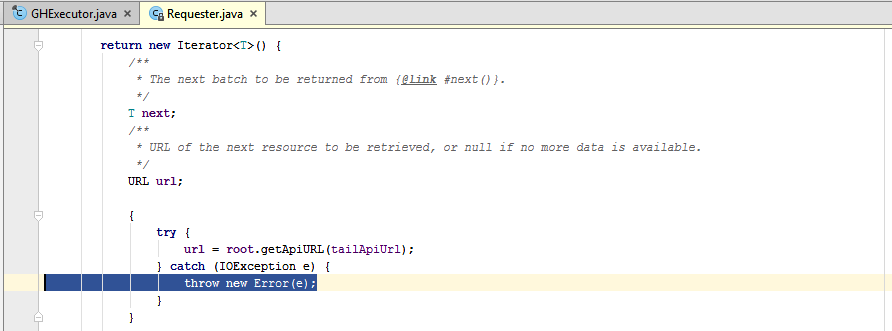
\includegraphics[width=400px]{kod_error1}
    \caption{Listing kodu źródłowego: nieoczekiwany błąd (Error) podczas połączeń z GitHub API}
    \label{koderr1}
\end{figure}


\begin{figure}[!h]
\centering
    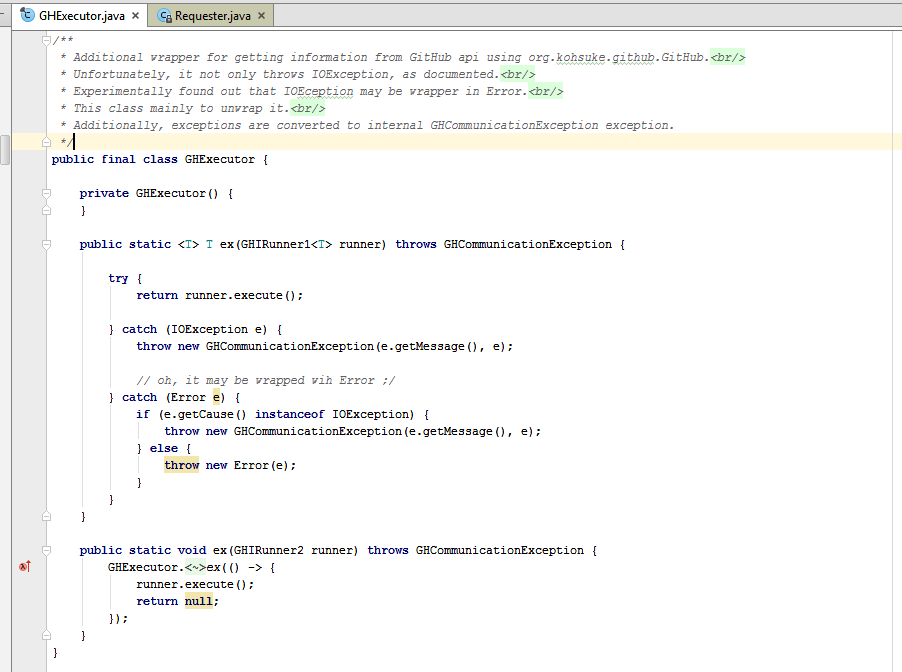
\includegraphics[width=\textwidth]{kod_error2}
    \caption{Listing kodu źródłowego: klasa GHCommunicationException}
    \label{koderr2}
\end{figure}

\section{Pamięć podręczna dla połączeń z~GitHub API}
Połączeń do GitHub API nie można wykonywać dowolnie dużo. GitHub limituje liczbę połączeń na godzinę. Limit ten dla połączeń anonimowych wynosi 60, natomiast dla połączeń używających danych autoryzacyjnych 5000 \cite{GitHubApiDoc}. Limit jest więc bardzo duży - wystarczy się przedstawić, a~można wysyłać zapytania o~zasoby częściej niż co sekundę. Teoretycznie można się nim nie przejmować limitem, i~nie wykonywać żadnych optymalizacji w~tym kierunku.

\medskip
Warto jednak pamiętać, że wykorzystujemy darmową usługę, i~chociażby w~ramach podziękowania zastosować się do wskazówek w~oficjalnej dokumentacji GitHub API. Znajduje się tam informacja, że jeżeli zapytania są wysyłane z~użyciem mechanizmów pamięci podręcznej, to w~ramach podziękowania w~pewnych przypadkach wykonanie zapytania nie obniża limitu. W~wielu odpowiedziach wysyłane są nagłówki HTTP \textquote{ETag} i/lub \textquote{Last-Modified}. Informacje te pozwalają wysłać żądanie warunkowe - \textquote{Podaj mi proszę zasób, tylko jeżeli się zmienił. W~przypadku braku zmian użyję odpowiedzi zapisanej w~pamięci podręcznej}. Jeżeli odpowiedzią na takie zapytanie warunkowe jest kod \textquote{304 Not Modified}, czyli \textquote{brak zmian}, to limit nie jest obniżany.

\medskip
Podążając wskazówkami autor postanowił dostosować swój kod, tak, by z~takiej pamięci podręcznej korzystał. W~dokumentacji biblioteki wykorzystywanej implementacji dostępu do GitHub API w~języku java - tj. \textquote{org.kohsuke: github-api}, znajduje się się rekomendacja zmiany domyślnego agenta http, na bibliotekę \textquote{OkHttp}, która obsługuje mechanizm pamięci podręcznej. Tak też zrobiono. Włączenie mechanizmu pamięci podręcznej spowodowało jednak, że algorytm kopiowania przestał działać poprawnie - nagle bardzo spowolnił, ilość zapytań paradoksalnie nie zmalała, a~wzrosła.

\medskip
Zapisywane informacje z~przebiegu działania algorytmu nie wskazywały jasno przyczyny. Ich analiza wykazała jednak, że przestój następował w~momencie odpytywania GitHub API o~informację, czy wysyłana gałąź w~repozytorium już jest widoczna jako zasób, co terminuje iż jej wysyłanie zakończyło się. Autor wysnuł teorię, że interfejs programistyczny usługi GitHub się myli, i~odpowiada niezgodnie z~rzeczywistością w~przypadku wysyłania zapytań warunkowych. Teoria ta znalazła potwierdzenie w~trakcie niezależnych prób z~użyciem ręcznie wysyłanych zapytań narzędziem cURL - okazało się, że zapytanie z~użyciem nagłówka \textquote{ETag} działa prawidłowo, ale dla \textquote{Last-Modified} informacja już jest błędna. Autor zgłosił błąd, a~programista GitHub potwierdził jego istnieje i~utworzenie w~wewnętrznym systemie zgłoszenia. Poinformował także, że nagłówek ten nie powinien być w~ogóle w~tym miejscu obsługiwany.

\medskip
Nie chcąc rezygnować z~pamięci podręcznej, w~tym momencie wydawało się jasne, że należy zmienić konfigurację biblioteki \textquote{OkHttp}, tak by dostosować priorytet używania nagłówków. Analiza dokumentacji i~kodu źródłowego tej biblioteki wykazała jednak, że obsługa nagłówka \textquote{ETag} ma priorytet przed nagłówkiem \textquote{Last-Modified}, więc wszystko powinno być w~porządku. Debugowanie aplikacji przy użyciu aplikacji Charles Proxy, tj. podsłuchując wykonywane połączenia HTTP w~systemie, wykazało, że prawdopodobnie GitHub API nie odpowiada nieprawidłowo. Właściwie to w~ogóle nie odpowiada, gdyż nie może - żadne zapytanie http nie zostało do niego wysłane.

\medskip
Ostatecznie okazało się, że GitHub API wysyła w~odpowiedzi nagłówek \textquote{Cache-Control: private, max-age=60, s-maxage=60}. Nagłówek ten informuje agenta http, że uzyskana odpowiedź pozostaje aktualna przez następne 60 sekund, i~nie ma powodu, by w~tym czasie wysyłać to zapytanie jeszcze raz. Używany agent http - OkHttp - prawidłowo obsługuje ten nagłówek, i~dostając żądanie o~ten sam zasób w~ciągu 60 sekund od jego zapamiętania, w~ogóle nie wykonuje połączenia, tylko od razu pobiera informację z~pamięci podręcznej. Dla algorytmu kopiującego informacja sprzed kilku sekund nie jest świeża, należy bezwzględnie zapytać o~aktualność zasobu dostawcę, tj. usługę GitHub. Nadpisanie tego nagłówka własną wartością rozwiązało problem.

\medskip
Debugując ten problem autor zupełnie przez przypadek znalazł błąd w~interfejsie programistycznym usługi GitHub. Błąd, chociaż istnieje, nie miał wpływu na faktyczną przyczynę spowolnienia algorytmu. Jest to ciekawe doświadczenie ukazujące, że nawet starannie wykonany zapis przebiegu działania algorytmu nie zawsze dostarcza poszukiwanej informacji. Nie oznacza to jednak, że takich zapisów nie należy dokonywać - bardzo ułatwiają one debugowanie aplikacji, a~przetoczoną historię należy traktować w~kategorii wyjątku potwierdzającego regułę.

\section{Relacja dziedziczenia po stronie bazy danych}
Inny warty zanotowania problem autor znalazł w~trakcie implementacji systemu formularzy. Jest to błąd z~kategorii heisenbug (za Wikipedia: \textquote{rodzaj błędu programu komputerowego, który wymyka się próbom wyizolowania warunków jego występowania, na przykład nie występuje lub daje inne rezultaty w~trakcie próby powtórzenia go w~tych samych warunkach} \cite{Heisenbug}).

\medskip
Moduł odpowiedzialny z~formularze operuje między innymi na takich encjach jak: Question, Input, InputText, InputScale. Question jest encją odpowiedzialną za przechowywanie szczegółów danego pytania, pozostaje ona w~relacji jeden do wielu z~encją Input. Encja Input natomiast jest typem abstrakcyjnym - przechowuje informacje wspólne dla wszystkich typów dostępnych form odpowiedzi. Encje InputText i~InputScale uszczegóławiają ten typ abstrakcyjny, i~są odpowiedzialne za konkretne typy formy odpowiedzi: odpowiednio komentarz tekstowy, i~ocena w~skali.

\medskip
Problem wynika z~połączenia wczytywania leniwego (ang. lazy) i~relacji dziedziczenia po stronie bazy danych. Z~jakiegoś powodu w~jednym z~miejsc otrzymywany typ Input wyrażał jedynie abstrakcyjną encję Input, nie był natomiast żadnym z~typów szczegółowych. Próba debugowania tego błędu była niemożliwa - ustawienie punktu stopu naprawiało problem - otrzymywany Input był typu szczegółowego.  Autor nie znalazł przyczyny takiego zachowania, nie wiadomo dlaczego w~trakcie próby debugowania błąd nie istniał. Nie może być to błąd typu race conditition, gdyż problem dotyczy otrzymanego typu otrzymanego obiektu.

\medskip
Pierwszą dokonaną próbą naprawy sytuacji było wyłączenie odczytu leniwego z~bazy, i~zastąpienie go chciwym (ang. eager). Mimo, że jest to bardzo skuteczne rozwiązania, to wyjątkowo słabe. Ilość dokonywanych zapytań do bazy danych diametralnie wzrosła. Taki spadek wydajności nie był do zaakceptowania.

\medskip
Ostatecznie problem został ominięty poprzez wykonanie inicjalizacji obiektu i~dokonanie jego konwersji na typ \textquote{prawdziwy}, zamiast operować na obiekcie typu \textquote{proxy} dostarczanego przez silnik dokonujący mapowania relacyjno-obiektowego. Zmiana ta została dodana do akcesora listy encji tupu Input w~encji Question. Po tej zmianie system działa prawidłowo, i~relacja dziedziczenia nie dostarcza problemów. Nie jest to jednak wyjaśnienie dlaczego bez tego występują problemy, i~gdzie faktycznie znajduje się błąd. Próba powtórzenia na prostszym, minimalistycznym projekcie się nie powiodła. Autor zrezygnował z~poszukiwania źródeł problemu z~ramach wykonywania pracy inżynierskiej, zastosowane rozwiązanie uznał za zadowalające.


% ex: set tabstop=4 shiftwidth=4 softtabstop=4 noexpandtab fileformat=unix filetype=tex spelllang=pl,en spell:
